%%%%%%%%%%%%%%%%%%%% author.tex %%%%%%%%%%%%%%%%%%%%%%%%%%%%%%%%%%%
%
% sample root file for your "contribution" to a contributed volume
%
% Use this file as a template for your own input.
%
%%%%%%%%%%%%%%%% Springer %%%%%%%%%%%%%%%%%%%%%%%%%%%%%%%%%%


% RECOMMENDED %%%%%%%%%%%%%%%%%%%%%%%%%%%%%%%%%%%%%%%%%%%%%%%%%%%
\documentclass[graybox]{svmult}

% choose options for [] as required from the list
% in the Reference Guide

\usepackage{mathptmx}       % selects Times Roman as basic font
\usepackage{helvet}         % selects Helvetica as sans-serif font
\usepackage{courier}        % selects Courier as typewriter font
%\usepackage{type1cm}        % activate if the above 3 fonts are
                            % not available on your system
%
\usepackage{makeidx}         % allows index generation
\usepackage{graphicx}        % standard LaTeX graphics tool
                             % when including figure files
\usepackage{multicol}        % used for the two-column index
\usepackage[bottom]{footmisc}% places footnotes at page bottom

% see the list of further useful packages
% in the Reference Guide

\makeindex             % used for the subject index
                       % please use the style svind.ist with
                       % your makeindex program

%%%%%%%%%%%%%%%%%%%%%%%%%%%%%%%%%%%%%%%%%%%%%%%%%%%%%%%%%%%%%%%%%%%%%%%%%%%%%%%%%%%%%%%%%

\begin{document}

\title*{The Hubness Phenomenon in High Dimensional Spaces}
% Use \titlerunning{Short Title} for an abbreviated version of
% your contribution title if the original one is too long
\author{Name of First Author and Name of Second Author}
% Use \authorrunning{Short Title} for an abbreviated version of
% your contribution title if the original one is too long
\institute{Name of First Author \at Name, Address of Institute, \email{name@email.address}
\and Name of Second Author \at Name, Address of Institute \email{name@email.address}}
%
% Use the package "url.sty" to avoid
% problems with special characters
% used in your e-mail or web address
%
\maketitle

\abstract*{Each chapter should be preceded by an abstract (10--15 lines long) that summarizes the content. The abstract will appear \textit{online} at \url{www.SpringerLink.com} and be available with unrestricted access. This allows unregistered users to read the abstract as a teaser for the complete chapter. As a general rule the abstracts will not appear in the printed version of your book unless it is the style of your particular book or that of the series to which your book belongs.
Please use the 'starred' version of the new Springer \texttt{abstract} command for typesetting the text of the online abstracts (cf. source file of this chapter template \texttt{abstract}) and include them with the source files of your manuscript. Use the plain \texttt{abstract} command if the abstract is also to appear in the printed version of the book.}

\abstract{Each chapter should be preceded by an abstract (10--15 lines long) that summarizes the content. The abstract will appear \textit{online} at \url{www.SpringerLink.com} and be available with unrestricted access. This allows unregistered users to read the abstract as a teaser for the complete chapter. As a general rule the abstracts will not appear in the printed version of your book unless it is the style of your particular book or that of the series to which your book belongs. \newline\indent
Please use the 'starred' version of the new Springer \texttt{abstract} command for typesetting the text of the online abstracts (cf. source file of this chapter template \texttt{abstract}) and include them with the source files of your manuscript. Use the plain \texttt{abstract} command if the abstract is also to appear in the printed version of the book.}

\section{Introduction}
\label{sec:1}
[Describe the phenomenon, recent observations, and open questions we are investigating here]



\section{Background and Related Work}
\label{sec:2}
% Always give a unique label
% and use \ref{<label>} for cross-references
% and \cite{<label>} for bibliographic references
% use \sectionmark{}
% to alter or adjust the section heading in the running head



\section{Intrinsic Dimensionality via Hubness}
\label{sec:3}

\subsection{Skewness vs. Feature Ranking - What is the Right Way to Rank Features? }
\label{subsec:3.1}
[Local Skewness plots, etc.]

\subsection{Supervised vs. Unsupervised Methods }
\label{subsec:3.2}
[Compare methods for feature relevance, cluster properties in original and subspace, etc.]


\section{Hubs, Density, and Clustering}
\label{sec:4}

To investigate the relationship between density hubness scores, and clustering, data sets of 30, 60, and 100 relevant dimensions were created. For each of these dimensions, two types of data sets were generated: (1) two Gaussian spheres separated by 10 units in the first coordinate and (2) two uniform cubes separated by one unit along its first dimension. In order to emulate varying densities, one cluster was designed to contain 1000 points and the second varied in size (2000, 3000, 4000, and 5000). There was a resulting total of 24 data sets given the different dimensions, distribution of points, and varying densities. For the rest of the chapter, the Gaussian data sets will be denoted as $G_{d,N}$ and the uniform ones as $U_{d,N}$, where $d$ is the dimension and $N$ is the number of points. In general, any $d$-dimensional data of $N$ points will be denoted as $X_{d,N}$.

\subsection{Hubness and Data Density}
\label{sec:4.1}

The first question to be addressed is whether hubness scores and density are the same measure. One way to see this is by plotting density against hubness scores. Suppose that there is a low density area, high density area, a low hubness score area and a high hubness score area, shown in Fig. \ref{fig:DensHubInt}. Intuition dictates that if density and hubness score were the same, all the points will lie within the first (high density and high hubness scores) and third (low density and low hubness scores) quadrants. If density and hubness score were the opposite, all the points will lie within the second (low density and high hubness scores) and fourth (high density and low hubness scores) quadrants. However, if the points are all over the four quadrants, then it might be telling of a different relationship between density and hubness scores. 

\begin{figure}
\centering
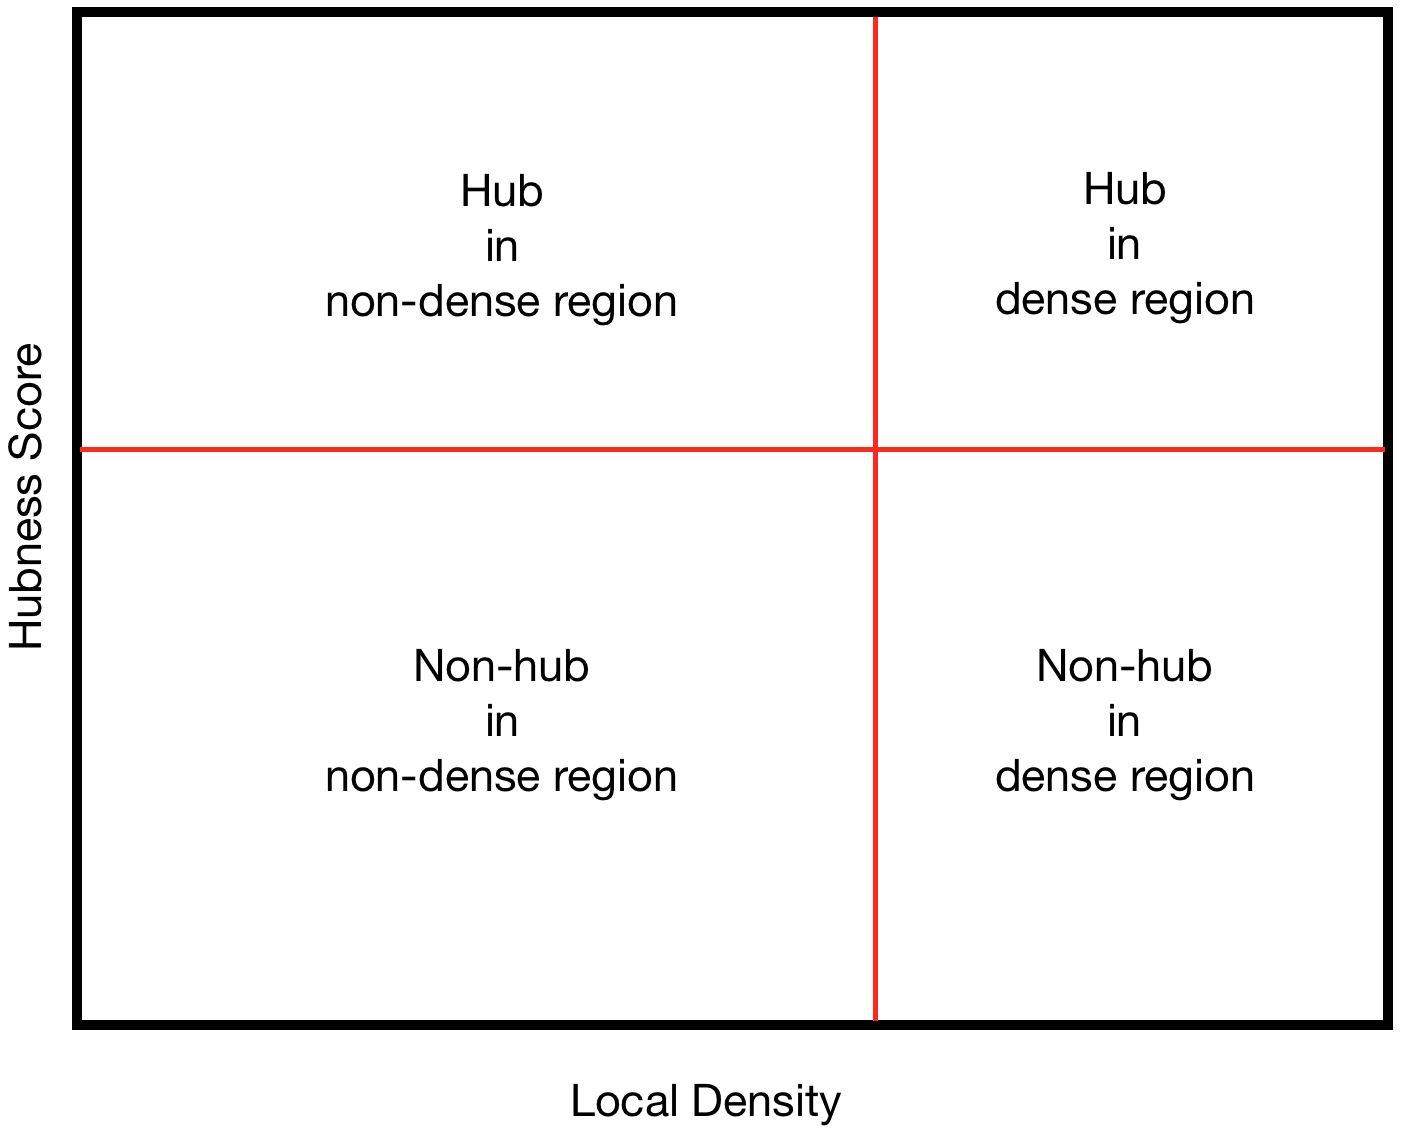
\includegraphics[width=2in,height=2in]{../fig/DensHub-Intuition.png}
\end{figure}\label{fig:DensHubInt}

For the experiments, the hubness scores $N_k$ were calculated for all the points with $k=5,10,$ and $50$. As far as the density estimation, $q_k(x) = \frac{1}{||x-x_k||}$, where $x$ is a data point and $x_k$ is the $k$th nearest neighbor of $x$, was chosen for its efficiency and since more sophisticated non-parametric consistent density estimators also suffer from the curse of dimensionality. All the density estimation plots used $q_{16}$. To determine what is ``high density'' and ``high hubness score,'' a threshold value of two standard deviations above the mean was calculated. A global threshold value, meaning that $N_k$ and $q_{16}$ were calculated for all the points regardless of class membership and then averages and standard deviations were calculated, can be seen in Fig.\ref{fig:GlobDensHubs}. 

\begin{figure}
\centering
    \begin{tabular}{cccc}
        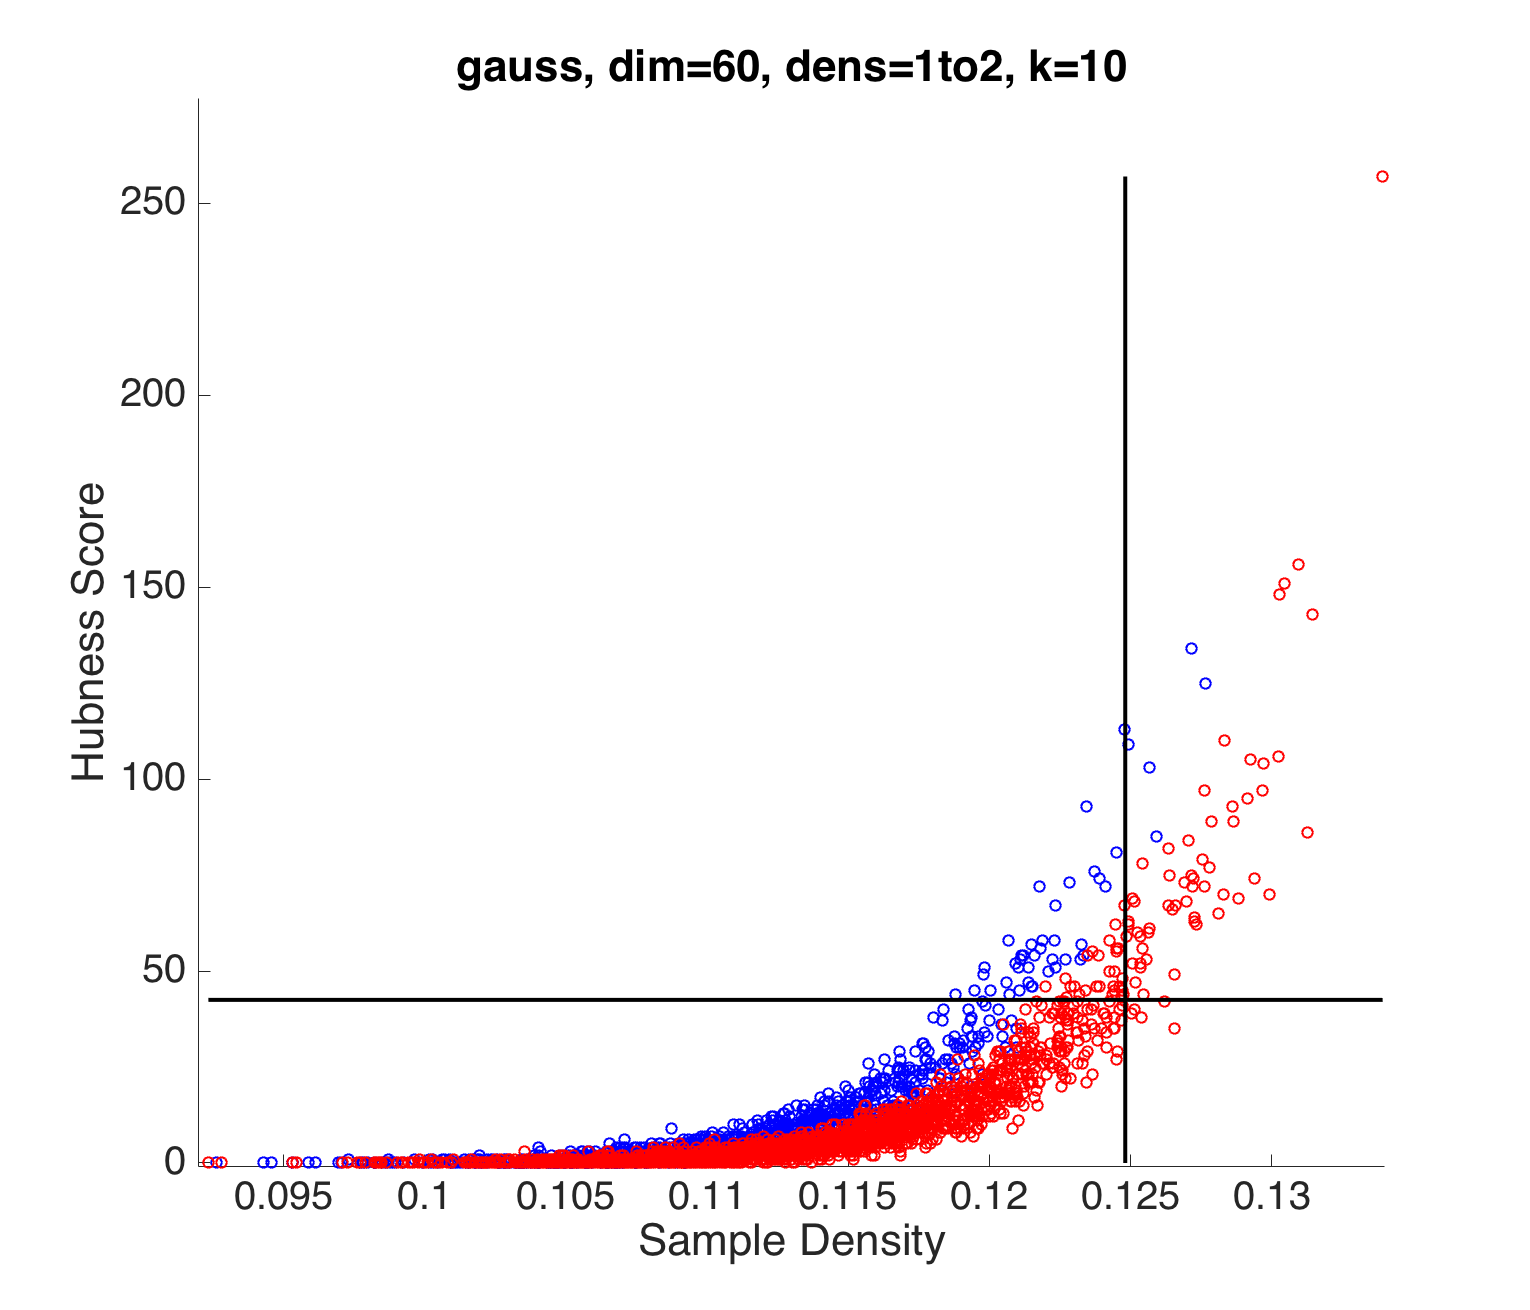
\includegraphics[width=2.5in,height=2in]{../fig/gauss-dim60-1to2-k10-GlobDensGlobHubs.png} &
        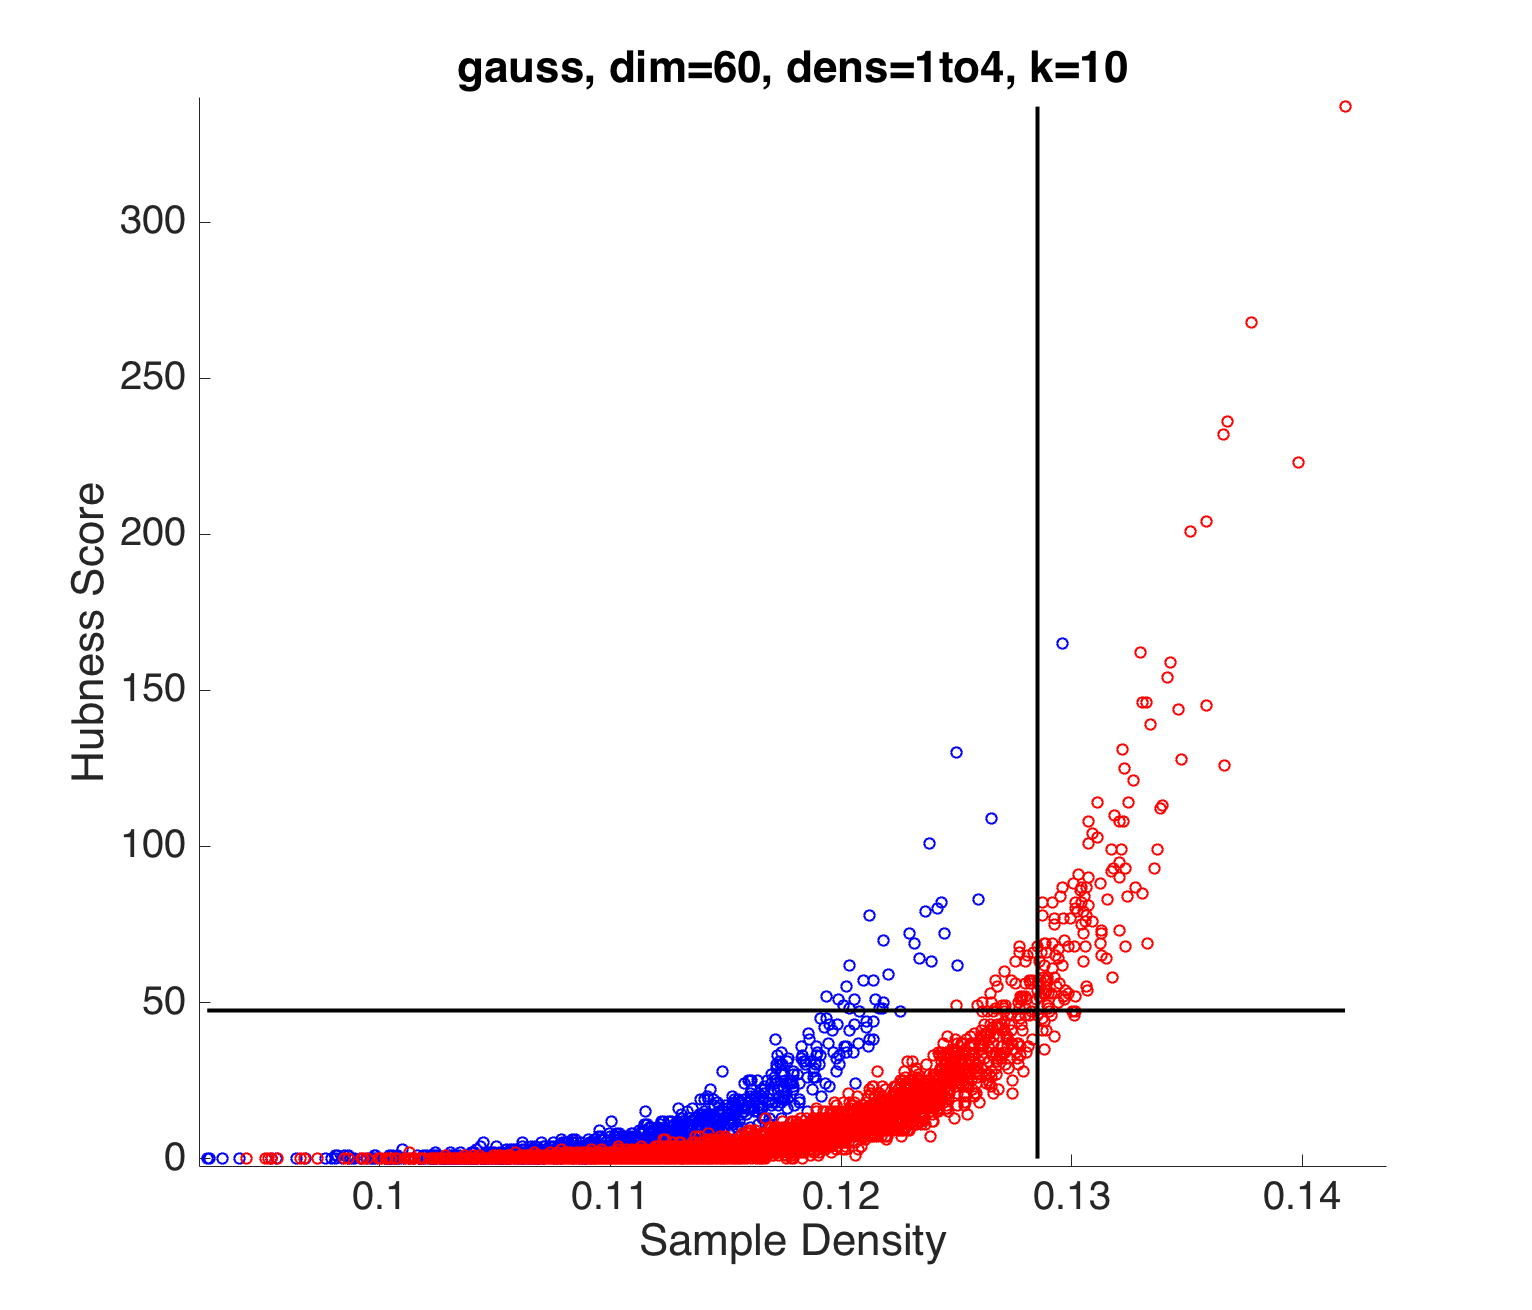
\includegraphics[width=2.5in,height=2in]{../fig/gauss-dim60-1to4-k10-GlobDensGlobHubs.png} \\
        {\scriptsize (a)} &  {\scriptsize (b)} \\
        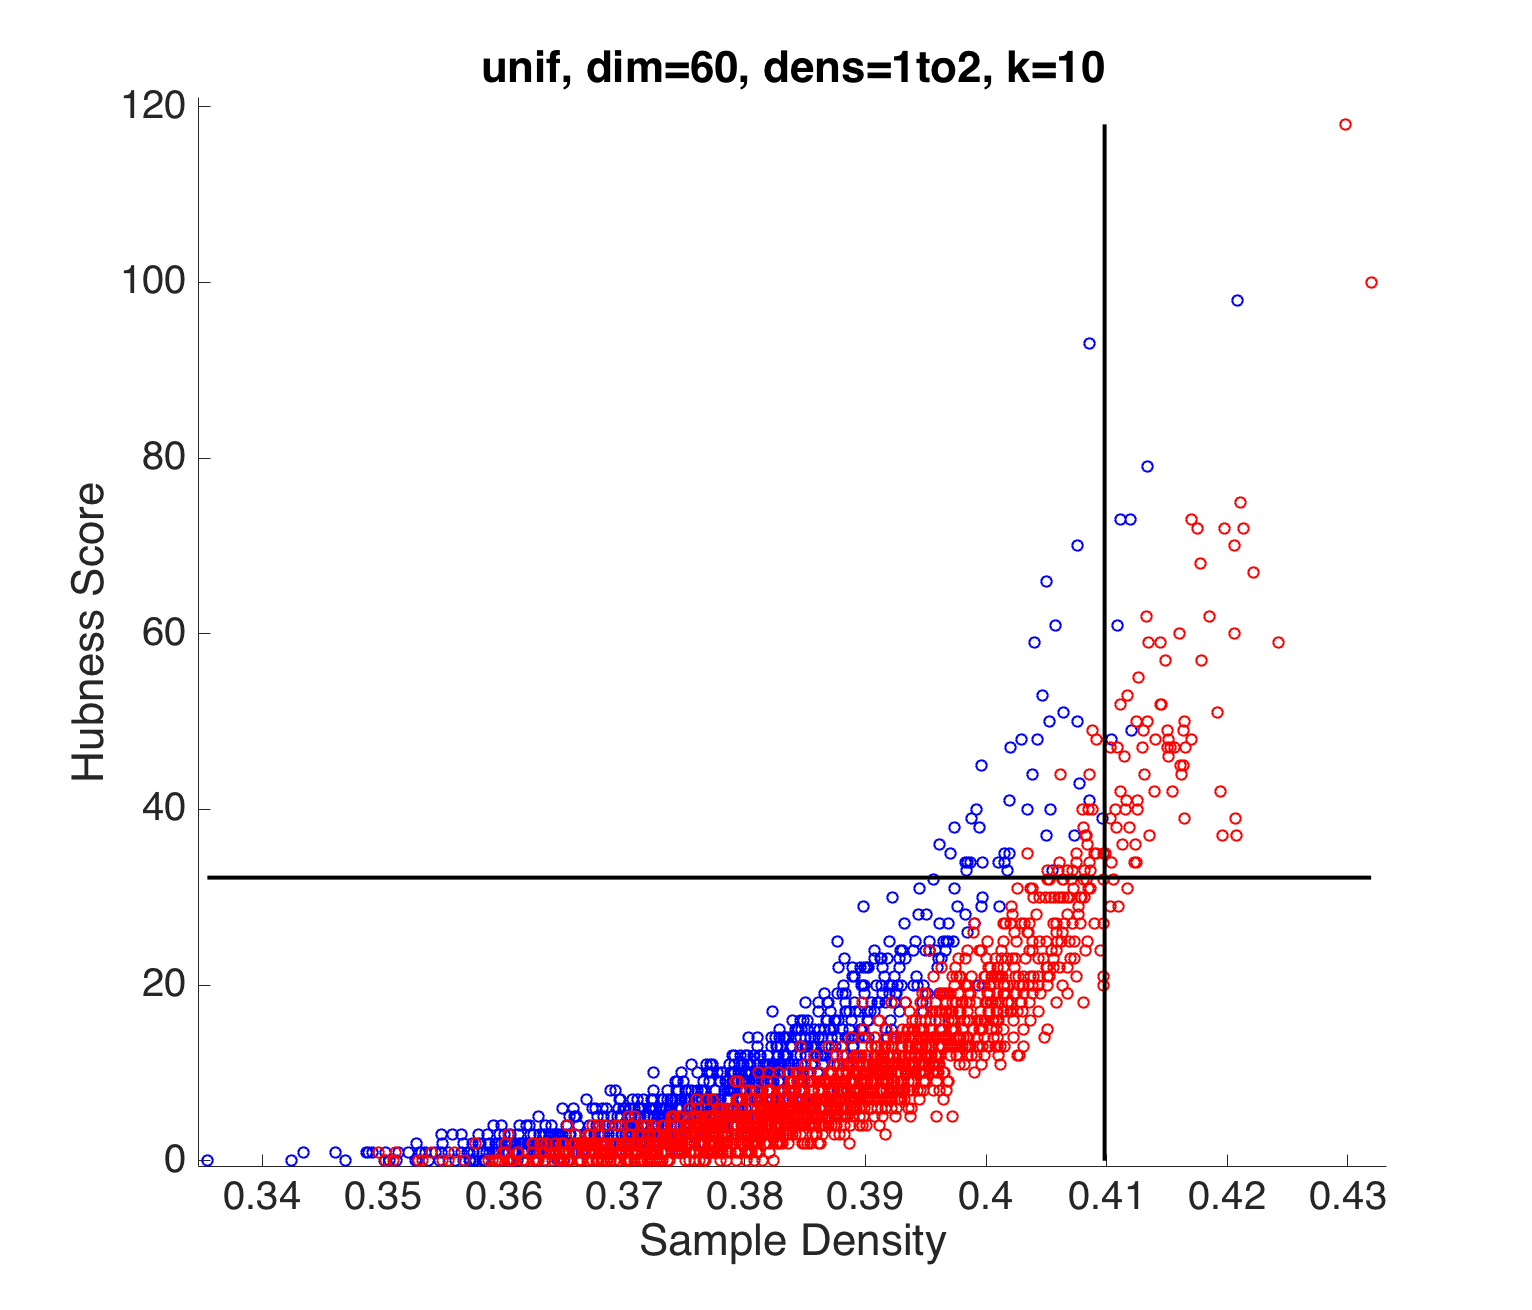
\includegraphics[width=2.5in,height=2in]{../fig/unif-dim60-1to2-k10-GlobDensGlobHubs.png}&
        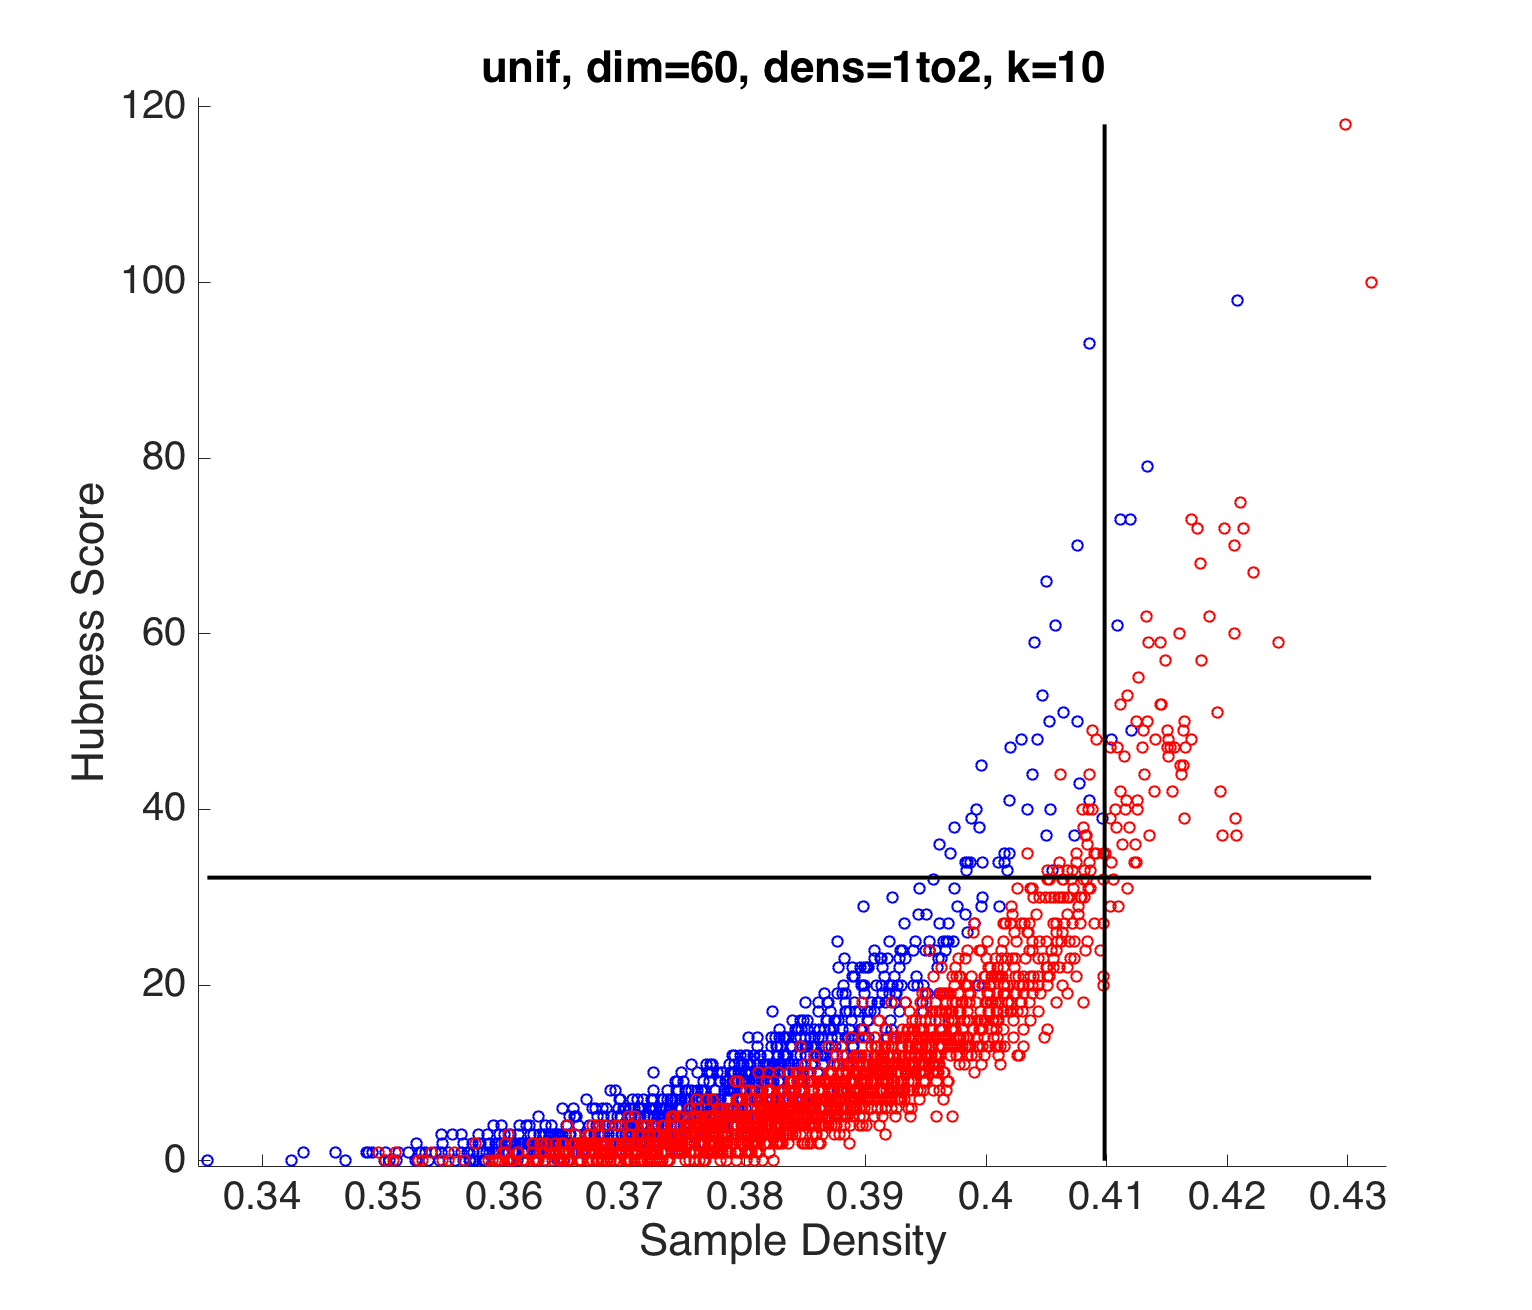
\includegraphics[width=2.5in,height=2in]{../fig/unif-dim60-1to2-k10-GlobDensGlobHubs.png}\\
        {\scriptsize (c)} &  {\scriptsize (d)} 
      \end{tabular}
      \caption{Density, $q_{16}$, plotted against hubness score, $N_{10}$, for data sets (a) $G_{60,3000}$, (b) $G_{60,5000}$, (c) $U_{60,3000}$, and (d) $U_{60,5000}$.}\label{fig:GlobDensHubs}
\end{figure}

[Distance plots, Correlation of hubs to density, etc.]

\subsection{Hubness and Clusters}
\label{sec:4.2}
        
[How do hubs relate to special points from various clustering methods (DBSCAN core points, outliers, etc.)?]

\subsection{Other Experiments PlaceHolder}
[These experiments could go into previous subsections as deemed fit:Landscape of hubs for different structured data, purity of reverse neighbors]

\section{Discussion}
\label{sec:5}



\section{Conclusion and Future Work}
\label{sec:6}

%\input{referenc}
\end{document}